%\documentclass[conference,spanish,a4paper,10pt,oneside,final]{IEEEtran}
%\nonstopmode
\documentclass[conference,a4paper,10pt,oneside,final]{tfmpd}


% esto me setea la variable pdf dependiendo del valor de \pdfoutput, que es >0
% sólo cuando estoy usando pdflatex para compilar el documento
\newif\ifpdf
\ifnum\pdfoutput<0
\pdffalse\fi
\ifnum\pdfoutput=0
\pdffalse\fi
\ifnum\pdfoutput>0
\pdftrue\fi

%\makeatletter
%\def\markboth#1#2{\def\leftmark{\@IEEEcompsoconly{\sffamily}\MakeUppercase{\protect#1}}%
%\def\rightmark{\@IEEEcompsoconly{\sffamily}\MakeUppercase{\protect#2}}}
%\makeatother


%
% ===
% === I18n / L10n
% ===
%
% babel me da separación de sílabas para palabras en el idioma que le paso como
%       argumento opcional. <-- Éste hay que pasarlo en \documentclass
%\usepackage{babel}
%
% inputenc define la codificación de caracteres del código fuente, acá utf8.
\usepackage[utf8]{inputenc}
%
% ===
% === Gráficos
% ===
% 
% pst-pdf me permite usar PSTricks con pdflatex. Necesito cargarlo sólo si está
%         definida la variable pdf, por eso está entre \ifpdf ... \fi
\ifpdf\usepackage{pst-pdf}\fi
%
% color me permite usar colores en el documento.
\usepackage{color}
%
% graphicx me da el comando \includegraphics para insertar imágenes (?)
\usepackage{graphicx}
%
% pstricks es un conjunto de macros basadas en PostScript para TeX, en
%          castellano, me da un entorno pstricks y comandos que uso dentro de
%          éste, que me sirven para dibujar figuras/diagramas/etc de manera
%          relativamente simple.
%\usepackage{pstricks}
%
% pst-circ me da macros para pstricks que me dibujan elementos de circuitos
%\usepackage{pst-circ}
%
% 
%\usepackage{pst-plot}		%Para dibujar una curva a partir de un archivo
%\usepackage{pst-2dplot}		%Para plotear. entorno pstaxes
%
% ===
% === Verbatims
% ===
%
% verbatim es una reimplementación de los entornos verbatim[*]
%          provee el comando \verbatiminput{archivo} y el entorno comment, que
%          hace que LaTeX ignore directamente todo lo que está adentro
%\usepackage{verbatim}
%
% moreverb implementa el entorno verbatimtab indentando los tabs que encuentre,
%          y también el entorno listing, que pone números de línea al verbatim.
%          Para cambiar el ancho de la tabulacion, uso
%          \renewcommand\verbatimtabsize{<ancho del tab>\relax}
%          También define el entorno boxedverbatim.
%\usepackage{moreverb}
%
% listings me da el entorno lstlisting con resaltado de sintaxis.
%          Para setear el lenguaje del código, hago \lstset{language=<lang>}
%\usepackage{listings}
%
% url es un verbatim para escribir URL's que permite linebreaks dentro de ésta.
%     para usarlo, \url{<URL>}
\usepackage{url}
%
%
%
%
%
%\usepackage{mdwlist}		%Para listas mas compactas
%\usepackage{textcomp}		%Para algunos símbolos
%\usepackage{colortbl}		%Para celdas de colores en tablas
%\usepackage{fancyhdr}		%Para encabezados/pie
%\usepackage{bbold}		%Fuente bb para modo math: \mathbb{R} = reales
%\usepackage{dsfont}		%Fuente ds para modo math: \mathds{R} = reales
\usepackage{multirow}		%Para "combinar" celdas en tablas
%\usepackage{float}		%Para cuadros, figuras, etc copadas
%\usepackage{fancybox}		%Para recuardos de texto con bordes "fancy"
%\usepackage{dingbat}		%Para dingbats
%%\usepackage{marginal}		%Para notas al margen que no puedo hacer andar
\usepackage{amsmath}		%Para enornos matemáticos mas flexibles
%\usepackage{varwidth}		%varwidth es un minipage que se ajusta al ancho mínimo
\usepackage{pslatex}            % setea fuentes Times, Helvetica y Courier ``angosta''

\usepackage[normalem]{ulem}     %para under/overlining. normalem hace que \emph se comporte como siempre

%

%Estilos de texto
\newcommand{\resalt}{\colorbox{green}}	%Resaltado - Fondo verde
\newcommand{\sfbf}{\bfseries\textsf}	%Slanted + Bold
\newcommand{\eng}{\textit}			%Palabra en inglés - Itálica
\newcommand{\mean}{\textsl}			%Significado de una sigla - Slanted
\newcommand{\defin}{\textbf}			%Definición - Negrita
\newcommand{\R}{\mathds}			%Para escribir R de Reales, N de Nat
\newcommand{\N}{\mathbf}			%Para escribir R de Reales, N de Nat
\newcommand{\lil}[1]{\footnotesize #1}
\newcommand{\mono}[1]{{\tt #1}}         % Monoespaciado


%Símbolos
\newcommand{\y}{\wedge}			%Y (Lógica)
\newcommand{\ve}{\vee}			%O (Lógica)
\newcommand{\ent}{\supset}		%Entonces (Lógica)
\newcommand{\dimp}{\leftrightarrow}	%Doble implicativo, equivalencia (Lógica)
\newcommand{\sii}{\leftrightarrow}	%Si y sólo si (Lógica)
\newcommand{\equi}{\equiv}		%Equivalencia (Lógica)
\newcommand{\portanto}{\vdash}	%Por lo tanto (Lógica)
\newcommand{\por}{\cdot}		%Producto punto

%Configuraciones del documento
%\selectlanguage{spanish}		%Elijo idioma español

%Tweaks
%\setlength{\parindent}{0mm}		%Sangría de 1a. línea
%\setlength{\hoffset}{-5.4mm}		%
%\setlength{\voffset}{-5.4mm}		%
%\setlength{\topmargin}{0mm}		%
%\setlength{\oddsidemargin}{5mm}	%
%\setlength{\evensidemargin}{5mm}	%
%\setlength{\marginparsep}{5mm}	%
%\setlength{\headheight}{12.5mm}	%
%\setlength{\headsep}{2.5mm}		%
%\setlength{\footskip}{10mm}		%
%\setlength{\textwidth}{15cm}		%
%\setlength{\textheight}{232mm}	%
%\setlength{\fboxrule}{.1pt}
%\setlength{\parskip}{.5\baselineskip}
%Colores
\definecolor{negro}	{cmyk}{0,0,0,1}
\definecolor{marron}	{cmyk}{0,.5,1,.41}
\definecolor{rojo}	{cmyk}{0,1,1,0}
\definecolor{naranja}	{cmyk}{0,.35,1,0}
\definecolor{amarillo}	{cmyk}{0,0,1,0}
\definecolor{verde}	{cmyk}{1,0,1,0}
\definecolor{azul}	{cmyk}{1,1,0,0}
\definecolor{violeta}	{cmyk}{.45,1,0,0}
\definecolor{gris}	{cmyk}{0,0,0,.5}
\definecolor{blanco}	{cmyk}{0,0,0,0}
\definecolor{dorado}	{cmyk}{0,.16,1,0}
\definecolor{plateado}	{cmyk}{0,0,0,.25}

%Comandos personalizados
\newcommand{\T}{\textrm}%Para escribir texto común cuando en modo math

% Remarca un ``texto insertado'' en rojo. Necesita el backage color.
\newenvironment{ins}{\color{red}$>$}{$<$}
\newcommand{\iins}[1]{{\color{red}$>$#1$<$}}

% Tacha un texto. Depende del package ulem.
\newcommand{\tachar}{\sout}

% Tacha doble
\newcommand{\Tachar}[1]{\xout{\xout{#1}}}

%\newcommand{\}

%\begin{pspicture}
%\def\tierra(#1){%Para dibujar el símbolo de tierra en el entorno PSTricks
%	\rput(#1){
%		\psdot(0,0)
%		\psline(0,0)(0,-0.45)
%		\psline(-0.5,-0.45)(0.5,-0.45)
%		\psline(-0.35,-0.6)(0.35,-0.6)
%		\psline(-0.2,-0.75)(0.2,-0.75)
%	}%
%}
%\end{pspicture}

%\newcommand{\codigo}[2]{%Para generar un recuadro con código
%	%\setlength{\hrulewidth}{0.1pt}
%	\begin{flushleft}
%	\underline{#1}
%	\begin{tabular}{@{\quad}|l}
%		\begin{minipage}{.85\textwidth}\smallskip{#2}
%	\end{minipage}\end{tabular}\end{flushleft}%
%}

%\newcommand{\filecodigo}[1]{%Insertar código verbatim desde un archivo
%\codigo{#1}{\verbatiminput{#1}}}%Requiere el paquete verbatim
%\newcommand{\filecodigobis}[1]{{\verbatiminput{#1}}}%Requiere el paquete verbatim

%\newcommand{\grafico}[3][1]{%Para generar un plot de un archivo con coords.
%%\def\deequis=#1
%\begin{minipage}{0.5\textwidth}\begin{center}
%\begin{pspicture}(6,5)
%	\psgrid[subgriddiv=1,gridlabels=0pt,gridwidth=.1pt](1,3)(1,1)(6,5)
%	\psset{xunit=5cm,yunit=2cm}
%	\fileplot[linewidth=1pt,linecolor=blue,origin={0.2,1.5}]{#2}
%	\psset{xunit=1cm,yunit=1cm}
%	\psaxes[Dx=#1,dx=5,Oy=-1,Dy=1,dy=2]{-}(0.9,1)(6,5)
%	\rput(4,0.4){\textsl{#3}}
%\end{pspicture}\end{center}\end{minipage}}

%\newcommand{\aclaracion}[1]{%Dibuja un recuadrito aclaratorio
%\smallpencil\ \begin{minipage}{0.9\textwidth}
%\vspace*{6pt}{#1}\smallskip\end{minipage}}

%\newcommand{\consigna}[1]{%Consigna - Slanted
%\leftpointright\ \parbox[t]{0.9\textwidth}{\textsl{#1}\vspace{8pt}}}

%\newcommand{\pinterno}[2]{%Consigna - Slanted
%\left\langle #1 , #2 \right\rangle}

%\newcommand{\eqncode}[2]{%
%\begin{center}
%\begin{tabular}{l@{\hspace{0.5cm}}r}
%\begin{minipage}{.4\textwidth}
%\begin{equation*}
%#1
%\end{equation*}
%\end{minipage}
%&
%\fbox{\begin{minipage}{.4\textwidth}
%%\setlength{\parskip}{4mm}
%\filecodigobis{#2}
%\end{minipage}}
%\end{tabular}
%\end{center}
%}

%\newcommand{\eqncodeb}[2]{%
%\begin{center}\begin{tabular}{l@{\hspace{0.5cm}}r}
%\begin{minipage}{.4\textwidth}#1\end{minipage} &
%\fbox{\begin{minipage}{.4\textwidth}\filecodigobis{#2}\end{minipage}}
%\end{tabular}\end{center}}

%\newenvironment{matemcode}[1]{\newline
%\begin{tabular}{l@{\hspace{0.5cm}}r}
%\begin{minipage}{.4\textwidth}
%\parbox[t]{.4\textwidth}{\begin{equation*}#1\end{equation*}}\end{minipage}
%&\begin{Sbox}\begin{minipage}{.4\textwidth}}
%{\end{minipage}\end{Sbox}\fbox{\TheSbox}\end{tabular}\newline}

%\newenvironment{encuadrar}[1]{\begin{Sbox}\begin{varwidth}{#1\textwidth}}
%{\end{varwidth}\end{Sbox}\fbox{\TheSbox}}

%\newenvironment{enunciado}
%{\leftpointright\ \begin{varwidth}[t]{0.9\textwidth}\textsl}
%{\end{varwidth}\vspace{8pt}}

%\newenvironment{parboxenv}{\begin{Sbox}}
%{\end{Sbox}\parbox[t]{.9\textwidth}{\TheSbox}}

%\newenvironment{pvi}{\begin{equation*}\begin{cases}}
%{\end{cases}\end{equation*}}

% Escribe el texto que le paso como parámetro con letra de ancho fijo.
%\newcommand{\mono}[1]{{\tt #1}}

%\title{\titulo}
%\author{\autor}
%\date{\fecha}

%% si uso pdflatex, me setea las propiedades del pdf de salida
%\ifpdf\pdfinfo{/Title    (\tituloPDF)
%               /Author   (\autorPDF)
%               /Subject  (\asuntoPDF)
%               /Keywords (\clavesPDF)}\fi

%
\begin{document}
\title{Identificación de edificios y monumentos a partir de fotografías
tomadas con dispositivos móviles}
\author{Esteban C. Fornal, Christian N. Pfarher, Mauro J. Torrez\\
\textit{Trabajo práctico final de ``Procesamiento Digital de
Imágenes'', II-FICH-UNL.}}
\markboth{Procesamiento Digital de Imágenes: TRABAJO FINAL}{}
\maketitle
%
%
% %%%%%%%%%%%%%%%%%%%%%%%%%%%%%%%%%%%%%%%%%%%%%%%%%%%%%%%%%%%%%%%%%%%%%%%%%%%%%%
%
%
\begin{abstract}
Se presenta un método para la identificación de edificios y monumentos, a
partir de fotografías tomadas con la cámara de un dispositivo móvil.
Se extrae un vector de características {globales y locales} de cada imagen.
{Se identifica una imagen de entrada minimizando el error cuadrático medio
entre sus vectores de características y los de una base de datos de imágenes
conocidas.}
Se presentan dos técnicas para la extracción de
características, una basada en la transformada de Hough y otra que
utiliza estadísticas de los histogramas.
Se evalúa el desempeño de ambas técnicas por separado y en
conjunto, para una base de datos de prueba.
\end{abstract}
%
%
% %%%%%%%%%%%%%%%%%%%%%%%%%%%%%%%%%%%%%%%%%%%%%%%%%%%%%%%%%%%%%%%%%%%%%%%%%%%%%%
%
%
\begin{keywords}
Identificación de edificios, \eng{building recognition},
histograma, transformada de Hough, clasificación.
\end{keywords}
%
%
% %%%%%%%%%%%%%%%%%%%%%%%%%%%%%%%%%%%%%%%%%%%%%%%%%%%%%%%%%%%%%%%%%%%%%%%%%%%%%%
%
%
\section{Introducción}
\PARstart{E}{n} la actualidad, la gran difusión de los dispositivos móviles nos
permite llevar la información importante siempre con nosotros. Además, es muy
común utilizar nues\-tros celulares, PDAs, GPS para obtener
información desde cualquier lugar donde estemos, gracias a la proliferación de
redes de datos inalámbricas. Dado que una gran parte de estos dispositivos
posee una cámara
digital, surge la idea de utilizarla junto con las conexiones de datos para
obtener información acerca del lugar donde nos encontramos. Se presenta aquí
un método que combina técnicas de Procesa\-mien\-to Digital de Imágenes
orientadas en este sentido, que permite la
identificación de edificios, monumentos y otros puntos de interés, a partir
de una fotografía capturada con un dispositivo móvil.
%
%
% %%%%%%%%%%%%%%%%%%%%%%%%%%%%%%%%%%%%%%%%%%%%%%%%%%%%%%%%%%%%%%%%%%%%%%%%%%%%%%
%
%
\section{Método propuesto}
En el método propuesto se pone énfasis en la etapa de
extracción de carac\-te\-rís\-ti\-cas de la imagen, considerando
un método trivial de clasificación.
%\subsection{Extracción de características}
La extracción de características se realiza %\tachar{\tachar{en este trabajo}}
mediante dos técnicas diferentes:
\begin{enumerate}
\item transformada de Hough, y
\item estadísticas del histograma.
\end{enumerate}
%
%%%%%%%%%%%%%%%%%%%%%%%%%%%%%%%%%%%%%%%%%%%%%%%%%%%%%%%%%%%%%%%%%%%%%%%%%%%%%%%%
%
\subsection{Extracción de características mediante Transformada de Hough}
La transformada de Hough nos permite visualizar, a partir de una imagen de
bordes, los parámetros de aquellas rectas\footnote{El procedimiento es general,
sirve para cualquier geometría que se pueda expresar en términos de sus
parámetros. En este trabajo, se utiliza el espacio de los parámetros de las
rectas, el más sencillo.}
que son principales en la imagen.

Para la extracción de características con esta técnica se siguen los siguientes
pasos:
\begin{enumerate}
\item A partir de la imagen original, se obtiene su versión en escala de grises
      promediando los tres canales RGB, y se la escala a un tamaño normalizado.
\item Se obtiene una imagen de sólo bordes, aproximando la magnitud del
      gradiente según
      \begin{equation}
      \label{sob}
      \nabla f \approx |G_x| + |G_y|,
      \end{equation}
      donde $G_x$, $G_y$ son el resultado de aplicar los o\-pe\-ra\-do\-res
      gradiente  de Sobel \cite{gonzalez+woods} (fig. \ref{masksobel}) a la
      imagen.
      Finalmente se umbraliza esta imagen de bordes utilizando un parámetro $U$:
      \begin{equation}
      \label{umbral}
      f(I)=
      \begin{cases}
      0, & I\leq U\\
      255, & I > U
      \end{cases}
      \end{equation}
      {donde $I=I(x,y)$ es el valor de la intensidad en el punto $(x,y)$.}
\item Con la imagen de bordes umbralizada se calcula la trans\-forma\-da de
      Hough para rectas.
\item Se aplica un escalado (submuestreo) a la transformada obtenida, llevándola
      a un tamaño pequeño
      para obtener mayor tolerancia tanto en el parámetro angular
      $\theta$ como en el de distancia $\rho$.
\item Se toman los $N$ máximos de esta transformada y se guardan en el vector de
      características sus coordenadas $(\rho,\theta)$, mapeadas al rango
      $[-1,1]$, obteniendo así un vector de $2N$ valores.
\end{enumerate}
El proceso completo puede verse en la Fig. \ref{procesohough}.
\begin{figure}
\begin{center}
\begin{tabular}{|c|c|c|}
\hline -1 & -2 & -1 \\\hline 0 & 0 & 0 \\\hline 1 & 2 & 1 \\\hline
\end{tabular}
\begin{tabular}{|c|c|c|}
\hline -1 & 0 & 1 \\\hline -2 & 0 & 2 \\\hline -1 & 0 & 1 \\\hline
\end{tabular}
\end{center}
\caption{Máscaras de filtrado (operadores gradiente) de Sobel.}
\label{masksobel}
\end{figure}

\begin{figure}
\begin{center}
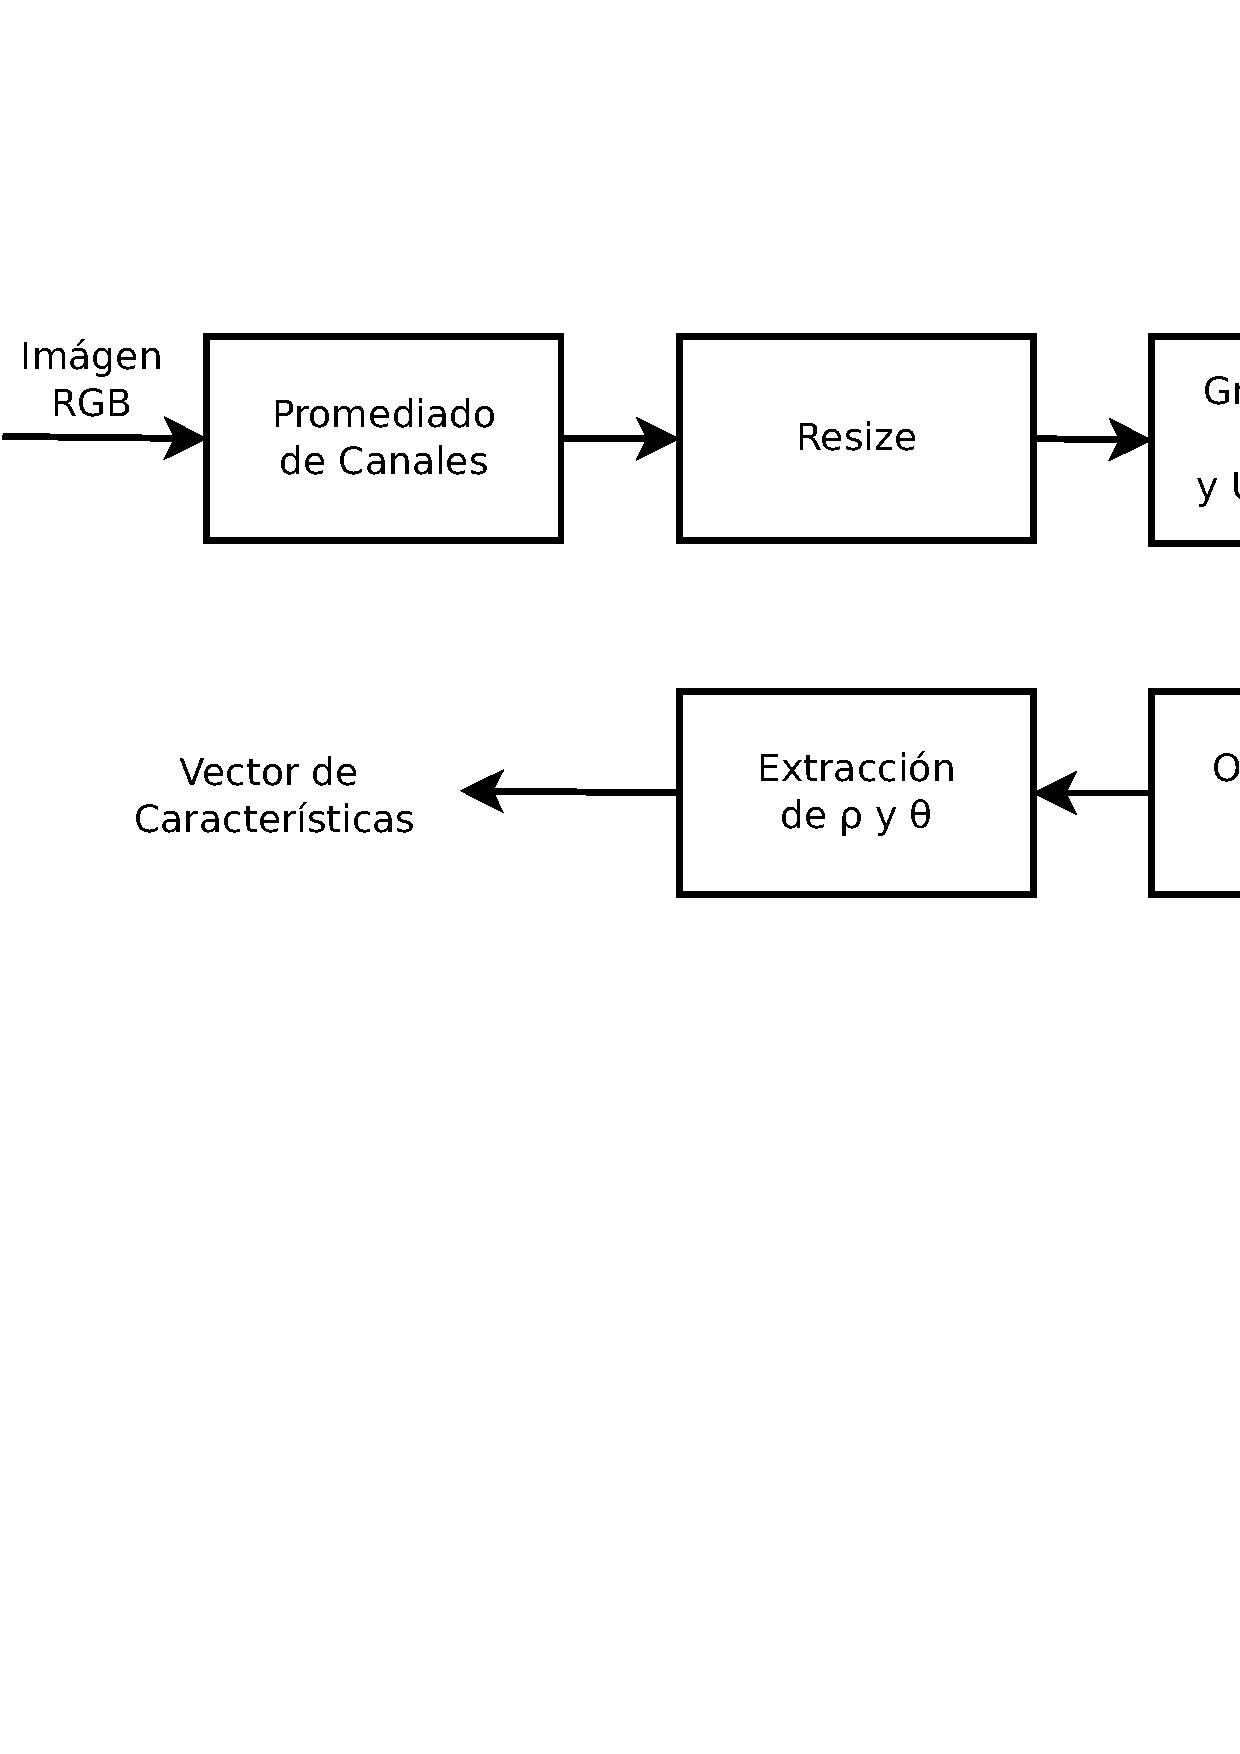
\includegraphics[scale=0.25]{../diagramas/procesohough} 
\end{center}
\caption{Proceso de extracción de características por Transformada de Hough}
\label{procesohough}
\end{figure}
%
%%%%%%%%%%%%%%%%%%%%%%%%%%%%%%%%%%%%%%%%%%%%%%%%%%%%%%%%%%%%%%%%%%%%%%%%%%%%%%%%
%
\subsection{Extracción de características por estadísticas del histograma}
A partir de la imagen original, se normaliza su tamaño y se toman 2
``perfiles de intensidad'': uno horizontal, calculado promediando
cada columna de la imagen, y otro vertical obtenido al promediar cada fila.
Estos ``perfiles'' se relacionan con la distribución de la energía promedio
en las filas y columnas de la imagen.
Luego se calculan tres histogramas, uno para cada perfil y otro para la
imagen entera. De estos 3 vectores, se calculan y se guardan en el
vector de características la media aritmética $m$, la mediana $M$ (posición del
percentil 50),  y la desviación absoluta $D_{\T{abs}}$ respecto de la mediana:
\begin{equation*}
D_{\T{abs}}=\sum_i |x_i - M|
\end{equation*}
Así, se ha obtenido un vector de 9 valores que caracterizan % histogramas de la
a la imagen entera.

Con la idea de incorporar características locales,
se sub\-di\-vi\-de la imagen en cuatro
cuadrantes y se obtienen, para cada uno, las mismas medidas que se calcularon
para  la imagen entera. Como resultado, se obtiene un vector de 45
características asociado a cada imagen.

\begin{figure}
\begin{center}
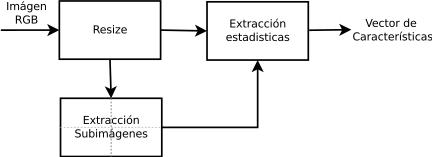
\includegraphics[scale=0.25]{../diagramas/procesoestadisticas}
\end{center}
\caption{Proceso de extracción de características utilizando estadísticas del
histograma.}
\label{procesoestadisticas}
\end{figure}

\subsection{Clasificación}
El entrenamiento de la base de datos se realiza obteniendo las características
para cada imagen, junto a su etiqueta.
Se extraen las características de todas las imágenes
con la misma etiqueta, y a partir de ellas se genera un
``prototipo'', que surge de promediar estas características.

La clasificación de las imágenes consiste en
obtener la e\-ti\-que\-ta del prototipo $p_{\T{ganador}}$ cuyas características
minimicen el error cuadrático medio con las de la imagen a identificar:
\begin{equation}
  p_{\T{ganador}}=\arg \min_i\left\{ \frac{1}{\sum N_j}
                \sum_{j=1}^K\sum_{n=0}^{N_j}(t_j[n]-p_{ij}[n])^2\right\}
\end{equation}
donde $t_j$ es el $j$-ésimo vector de características extraído de la imagen, con
longitud $N_j$, y $p_{ij}$ es el $j$-ésimo vector de características del
$i$-ésimo prototipo generado en el entrenamiento, también de longitud $N_j$.
%
%
%%%%%%%%%%%%%%%%%%%%%%%%%%%%%%%%%%%%%%%%%%%%%%%%%%%%%%%%%%%%%%%%%%%%%%%%%%%%%%%%
%
%
\section{Experimentos y resultados}
%
%%%%%%%%%%%%%%%%%%%%%%%%%%%%%%%%%%%%%%%%%%%%%%%%%%%%%%%%%%%%%%%%%%%%%%%%%%%%%%%%
%
\subsection{Base de datos}
La base de datos se armó con imágenes de prueba tomadas con teléfonos celulares
corrientes, a una resolución VGA estándar de 640 píxeles de ancho por 480 de
alto, en diferentes condiciones
de iluminación: día a pleno sol, día nublado, noche, e interior, a monumentos/%
estatuas y edificios en diferentes lugares de la ciudad de Santa Fe (Argentina).
{Se obtuvieron 195 imágenes, 13 por cada uno de los 15 prototipos diferentes en
total.}
Se muestran en la figura \ref{imagenes} dos ejemplos de las imágenes utlizadas.
%
%%%%%%%%%%%%%%%%%%%%%%%%%%%%%%%%%%%%%%%%%%%%%%%%%%%%%%%%%%%%%%%%%%%%%%%%%%%%%%%%
%
\subsection{Experimentación}
Se generaron 3 {casos} de prueba diferentes, tomando
5 etiquetas al azar (no repetidas) para cada {uno}.
Para la prueba del método {en cada caso} se utilizó validación cruzada,
entrenando la base de datos con 10 imágenes por etiqueta, y dejando las 3
imágenes restantes para la prueba.

\begin{figure}
\begin{center}
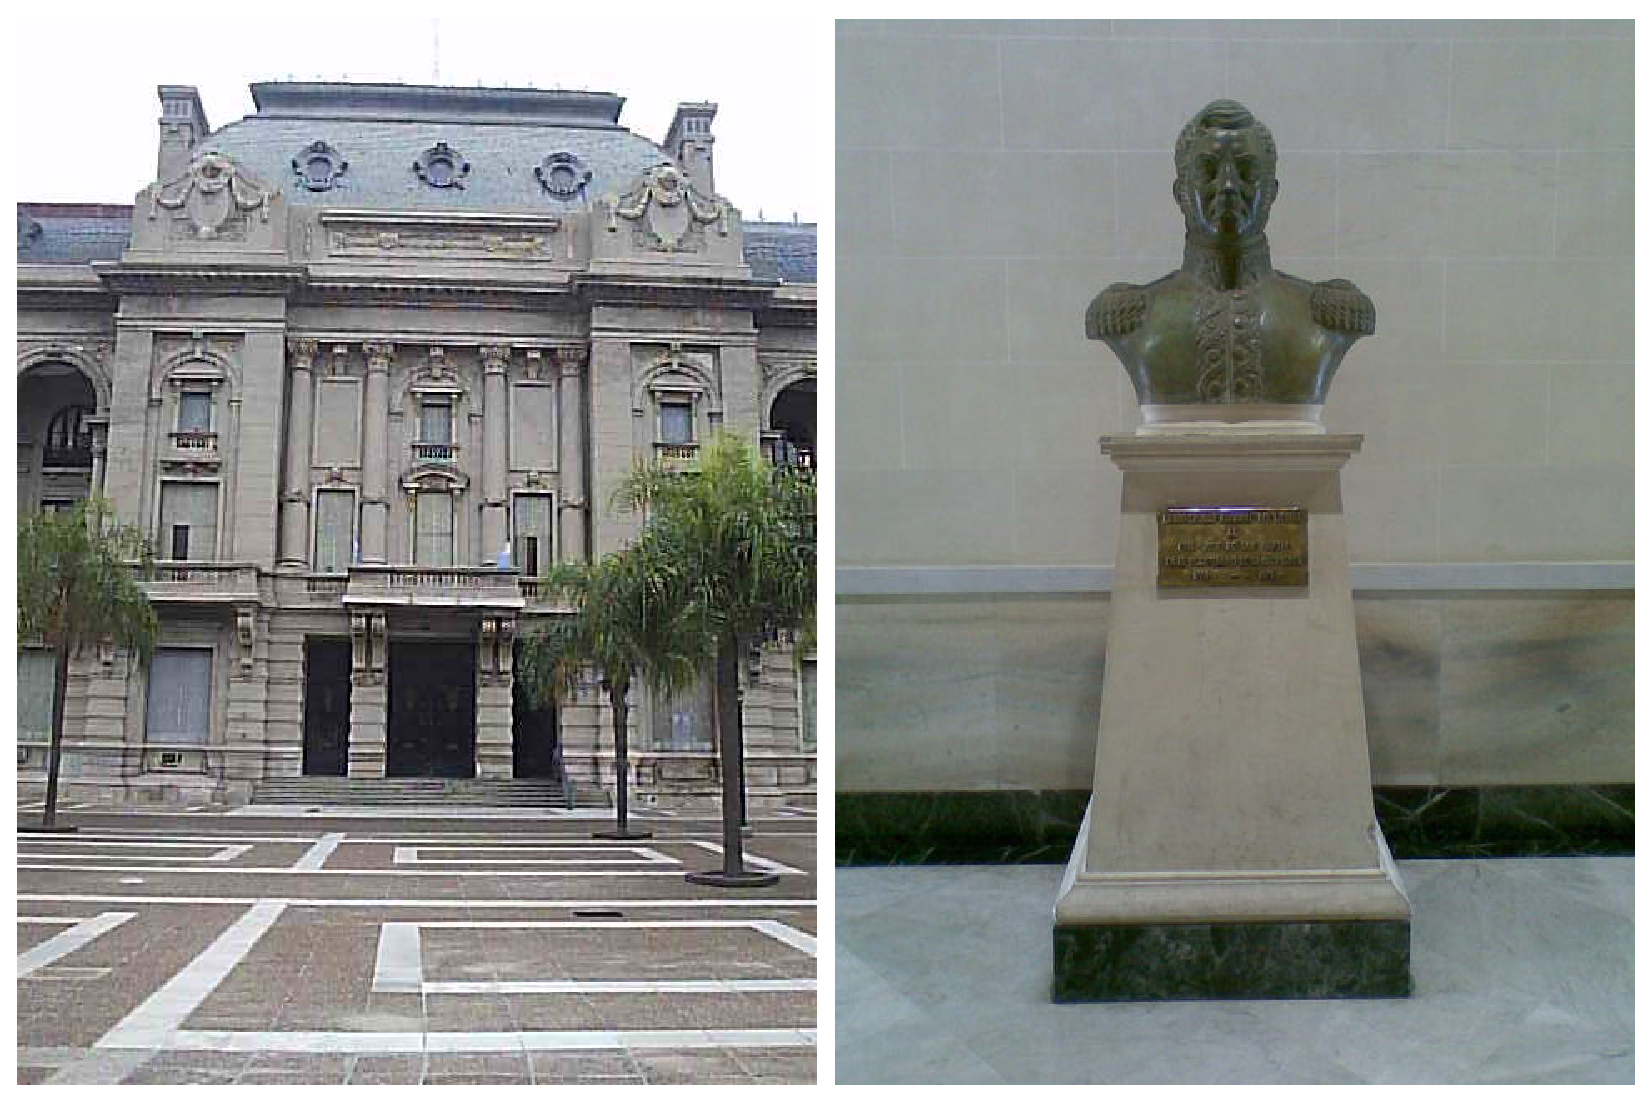
\includegraphics[scale=0.25]{../diagramas/dibujo}
\end{center}
\caption{Ejemplo de dos imágenes utilizadas para probar el método.}
\label{imagenes}
\end{figure}

Se clasificó utilizando extracción de características mediante
transformada de Hough y mediante histogramas por separado.
Para la técnica de Hough se probaron diferentes valores de $U$ (el umbral
aplicado a la imagen de bordes) y $N$ (el número de máximos considerados
en el espacio de la transformada de Hough); mientras que,
para el método de histograma se consideró el histograma y los perfiles
del canal de intensidad en el espacio de colores HSI.

Luego se evaluó el rendimiento del método utilizando todas las características
en forma conjunta, para los parámetros de Hough $U$ y $N$ óptimos encontrados.

Se realizó además un {caso de prueba} con las 15 etiquetas de
imágenes en conjunto, con el objetivo de tener una estimación de cómo responde
el método para un mayor número de imágenes.

Se considera la tasa de error ($\%$) del método según:
\begin{equation}
E_\%=100\cdot\frac{\T{número de errores}}{\T{número de pruebas}},
\end{equation}
considerando como error a cada prueba en que la imagen es mal etiquetada.

Cabe destacar que la clasificación se realiza en términos de clases, que
representan a un edificio/monumento en cualquier condición de iluminación
(puede haber varias etiquetas/prototipos que corresponden a la misma clase),
luego no es un error que la imagen de prueba se etiquete en forma incorrecta
si la clase es la acertada.
Por ejemplo, no es error si la imagen de un monumento tomada de día es
etiquetada como la del mismo monumento, pero tomada de noche.
Esta consideración se hace debido a que la detección de bordes elimina la
información de iluminación de la imagen, y está claro que no influye
en la técnica por histograma, ya que éste varía significativamente
entre las versiones de día y noche; en particular, la media y mediana tendrán
valores bastante menores en la imagen nocturna que en aquella tomada de día.
Esto es además consistente con el objetivo del método, que es la correcta
identificación de la clase (clasificación), independientemente de las
condiciones (etiqueta) en que se toma la imagen.
%
% %%%%%%%%%%%%%%%%%%%%%%%%%%%%%%%%%%%%%%%%%%%%%%%%%%%%%%%%%%%%%%%%%%%%%%%%%%%%%%
%
\subsection{Resultados}
Los resultados de las pruebas con {la técnica} de Hough se muestran en la figura
\ref{graficaerror}. Se ha tomado un rango de valores representativos de $U$
y $N$ basados en pruebas previas, donde hemos identificado regiones de mínimo
error para $U~\in(60,120)$ y $N~\in(20,60)$.
En la misma figura, se puede apreciar que la tasa de error mínima se obtuvo
para un umbral $U = 100$ y unos $N = 30$ máximos (en promedio).

\begin{figure}
\begin{center}
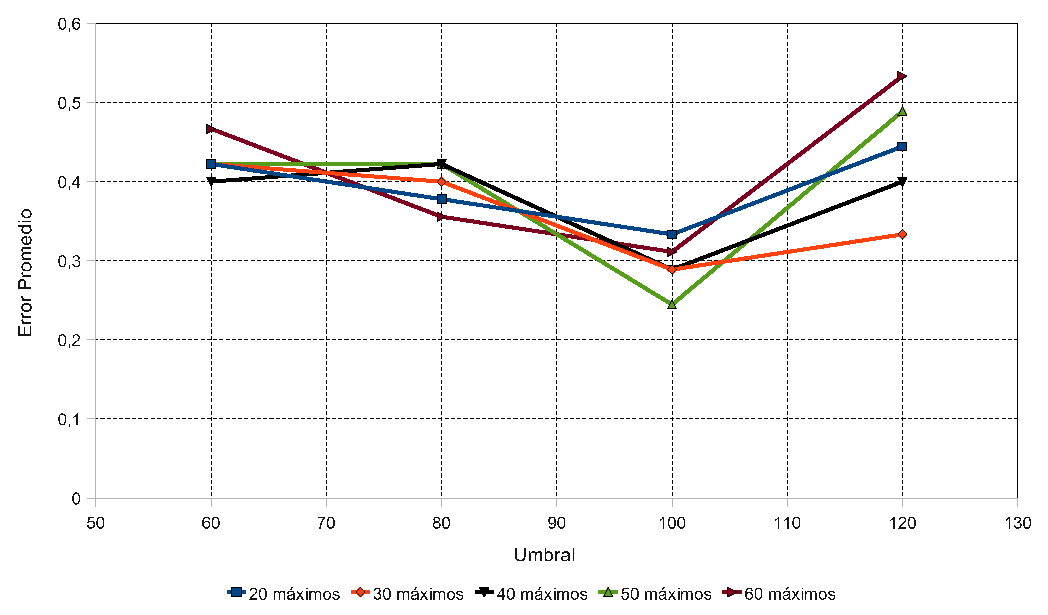
\includegraphics[width=8.5cm]{../diagramas/estadistica_noche_iguales}
\end{center}
\caption{Error de clasificación promedio en función de distintos $U$ y $N$ para
{la técnica} de Hough.}
\label{graficaerror}
\end{figure}

En la tabla \ref{tablaerrores} se presentan los resultados para
{los casos de prueba} de 5 etiquetas {y para el caso de} 15 etiquetas.
%
%Cabe aclarar que en el primer caso se tomó un promedio de los errores
%sobre el conjunto.
%
\begin{table}
\caption{Tasas de error para {las técnicas de extracción de características}.}
\begin{center}\begin{tabular}{ccc}
\hline \emph{{Técnica}} & \emph{5 etiquetas} & \emph{15 etiquetas}\\
\hline Histogramas & 0\% & 0\%\\
\hline Hough & 35.5\% & 60.43\%\\
\hline Histogramas+Hough & 2.22\% & 4.17\%\\
\hline
\end{tabular}\end{center}
\label{tablaerrores}
\end{table}
%
Se puede observar que para {la técnica} de histogramas,
la tasa de error fue cero
en ambas pruebas. En tanto que para {la} de Hough,se obtiene menor tasa de
error {en los casos} de 5 etiquetas que con el de 15, de 35.5\% y 60.43\%
respectivamente. En la última fila, se muestran los resultados de
con\-si\-de\-rar {ambas técnicas}
en conjunto, asignándole un peso equivalente a cada una.
%
% %%%%%%%%%%%%%%%%%%%%%%%%%%%%%%%%%%%%%%%%%%%%%%%%%%%%%%%%%%%%%%%%%%%%%%%%%%%%%%
%
\subsection{Discusión}
A pesar de la muy buena performance de la técnica de histograma, debemos tener
presente que las  imágenes de entrenamiento/prueba han sido obtenidas
en todos los casos a partir de una secuencia tomada en el
lapso de unos minutos, con el mismo dispositivo, lo cual implica que las
condiciones de iluminación en cada etiqueta --con la que luego se generan
los prototipos-- son prácticamente iguales.

Los histogramas miden la distribución estadística de los diferentes niveles
de intensidad presentes en la imagen, luego están estrechamente relacionados
con las condiciones de iluminación de la escena. Por este motivo, tenemos
que los histogramas entre las imágenes de entrenamiento/prueba son
similares, lo cual explica el buen funcionamiento de este método.

Se ha probado la técnica de histogramas sobre el canal I del espacio de color
HSI; por lo antes expuesto, debemos tener en cuenta consideraciones similares
para el resto de los canales de la imagen.

En general, se deberá poner énfasis en definir técnicas
de ``normalización'' orientadas a mejorar los resultados en condiciones más
realistas. Se deberá considerar la utilización de métodos de histograma
mejorados, por ejemplo el \emph{histograma de combinación espacial de DCT
ponderada} \cite{wdctsch}, \emph{vectores de coherencia de
color} \cite{Pass96histogramrefinement}, o el procesamiento de
histogramas borrosos presentado en \cite{Konstantinidis2005375}.

Respecto de la extracción de características mediante la transformada de Hough,
vemos que el rendimiento no es tan bueno como en la técnica de histogramas,
sin embargo en varios casos ha sido capaz de identificar correctamente
e\-di\-fi\-cios a pesar de las diferentes condiciones de
 iluminación (día y noche), lo cual es un resultado alentador.

No se puede evitar la mención al costo computacional del proceso, que aunque
no es tan elevado como para considerar impráctico el método, sí será una
limitante al considerar implementaciones en tiempo real o de alta velocidad
de respuesta: en una computadora promedio el cálculo se realiza en 1--2
segundos, luego es esperable que este tiempo se triplique en un
dispositivo móvil.

Se deberá considerar la utilización de un mejor detector de bordes, como el
propuesto por Canny \cite{canny},
así como también técnicas de pre-procesamiento de la
imagen, como puede ser el filtrado homomórfico, en pos de mejorar los
resultados obtenidos en nuestras pruebas.

En lo que respecta a la escalabilidad de la base de datos, los resultados no
son particularmente alentadores, lo que nos {podría estar
indicando que las características extraídas no son suficientemente \emph{únicas}
para las imágenes, obligándonos} a considerar otra vez la
utilización de métodos más refinados de histograma y transformada de Hough.
%
%
% %%%%%%%%%%%%%%%%%%%%%%%%%%%%%%%%%%%%%%%%%%%%%%%%%%%%%%%%%%%%%%%%%%%%%%%%%%%%%%
%
%
\section{Conclusiones}
Se ha presentado una técnica para la identificación de edificios, monumentos,
esculturas con extracción de características mediante medidas de histograma
y transformada de Hough.

El rendimiento ha sido satisfactorio considerando las restricciones a las
que se han sometido las pruebas.

Se debe optimizar la implementación para portarlo a dispositivos móviles
con capacidad de procesamiento limitada.

Se hace necesario un preprocesamiento de la imagen, así como la incorporación
de métodos más refinados de extracción de características, para mejorar los
resultados obtenidos y así poder usar el método con una base de datos de
mayor magnitud.
%
%
% %%%%%%%%%%%%%%%%%%%%%%%%%%%%%%%%%%%%%%%%%%%%%%%%%%%%%%%%%%%%%%%%%%%%%%%%%%%%%%
%
%
\section{Trabajos futuros}
A partir del diseño aquí presentado, han surgido líneas para continuar
investigando y lograr un método más robusto:
\begin{itemize}
\item Aplicación de filtrado homomórfico y otros tipos de
      pre-procesamiento en las imágenes.
\item Aplicación de técnicas de \eng{warping} y otras transformaciones en busca
      de lograr invarianza respecto de rotación y escalado de la imagen.
\item Desarrollo de técnicas de extracción de características más {refinadas}.
\item Desarrollo de una implementación óptima para dis\-po\-si\-ti\-vos
      móviles con poder de procesamiento limitado.
\end{itemize}
\nocite{*}
\bibliographystyle{tfmpd}
\bibliography{tfmpd}
\end{document}
